% Author: Izaak Neutelings (September 2021)
% Inspiration:
%   https://jila.colorado.edu/~ajsh/insidebh/penrose.html
%   https://tex.stackexchange.com/questions/99124/how-to-draw-penrose-diagrams-with-tikz
%   coordinates: https://arxiv.org/pdf/physics/0611033.pdf
%   https://arxiv.org/pdf/0711.0873.pdf
\documentclass[border=3pt,tikz]{standalone}
\usepackage{tikz}
\usepackage{amsmath} % for \text
\usepackage{mathrsfs} % for \mathscr
\usepackage{xfp} % higher precision (16 digits?)
\usepackage[outline]{contour} % glow around text
\usetikzlibrary{decorations.markings,decorations.pathmorphing}
\usetikzlibrary{angles,quotes} % for pic (angle labels)
\usetikzlibrary{arrows.meta} % for arrow size
\contourlength{1.4pt}

\newcommand{\calI}{\mathscr{I}} %\mathcal
\tikzset{>=latex} % for LaTeX arrow head
\colorlet{myred}{red!80!black}
\colorlet{myblue}{blue!80!black}
\colorlet{mygreen}{green!80!black}
\colorlet{mydarkred}{red!50!black}
\colorlet{mydarkblue}{blue!50!black}
\colorlet{mylightblue}{mydarkblue!6}
\colorlet{mypurple}{blue!40!red!80!black}
\colorlet{mydarkpurple}{blue!40!red!50!black}
\colorlet{mylightpurple}{mydarkpurple!80!red!6}
\colorlet{myorange}{orange!40!yellow!95!black}
\tikzstyle{cone}=[mydarkblue,line width=0.2,top color=blue!60!black!30,
                  bottom color=blue!60!black!50!red!30,shading angle=60,fill opacity=0.9]
\tikzstyle{cone back}=[mydarkblue,line width=0.1,dash pattern=on 1pt off 1pt]
\tikzstyle{world line}=[myblue!60,line width=0.4]
\tikzstyle{world line t}=[mypurple!60,line width=0.4]
\tikzstyle{particle}=[mygreen,line width=0.5]
\tikzstyle{photon}=[-{Latex[length=4,width=3]},myorange,line width=0.4,decorate,
                    decoration={snake,amplitude=0.9,segment length=4,post length=3.8}]
\tikzstyle{singularity}=[myred,line width=0.6,decorate,
                         decoration={zigzag,amplitude=2,segment length=6.17}]
\tikzset{declare function={%
  penrose(\x,\c)  = {\fpeval{2/pi*atan( (sqrt((1+tan(\x)^2)^2+4*\c*\c*tan(\x)^2)-1-tan(\x)^2) /(2*\c*tan(\x)^2) )}};%
  penroseu(\x,\t) = {\fpeval{atan(\x+\t)/pi+atan(\x-\t)/pi}};%
  penrosev(\x,\t) = {\fpeval{atan(\x+\t)/pi-atan(\x-\t)/pi}};%
  kruskal(\x,\c)  = {\fpeval{asin( \c*sin(2*\x) )*2/pi}};% Penrose coordinates for Kruskal
}}
\def\tick#1#2{\draw[thick] (#1) ++ (#2:0.04) --++ (#2-180:0.08)}
\def\Nsamples{20} % number samples in plot

% LIGHTCONE
\def\R{0.08} % size lightcone
\def\e{0.08} % vertical scale
\def\ang{45} % angle light cone
\def\angb{acos(sqrt(\e)*sin(\ang))} % angle ellipse center to point of tangency
\def\a{\R*sin(\ang)*sqrt(1-\e*sin(\ang)^2)/(1-\e*sin(\ang)^2)} % vertical radius
\def\b{\R*sqrt(\e)*sin(\ang)*cos(\ang)/(1-\e*sin(\ang)^2)} % horizontal radius
\def\coneback#1{ % light cone part to be drawn behind world lines
  \draw[cone back] % dashed line back
    (#1)++(-45:\R) arc({90-\angb}:{90+\angb}:{\a} and {\b});
  \draw[cone,shading angle=-60] % top edge & inside
    (#1)++(0,{\R*cos(\ang)/(1-\e*sin(\ang)^2)}) ellipse({\a} and {\b});
}
\def\conefront#1{ % light cone part to be drawn over world lines
  \draw[cone] % light cone outside
    (#1) --++ (45:\R) arc({\angb-90}:{-90-\angb}:{\a} and {\b})
     --++ (-45:2*\R) arc({90-\angb}:{-270+\angb}:{\a} and {\b}) -- cycle;
}

\begin{document}


% PENROSE DIAGRAM of Minkowski space - 45 rotation
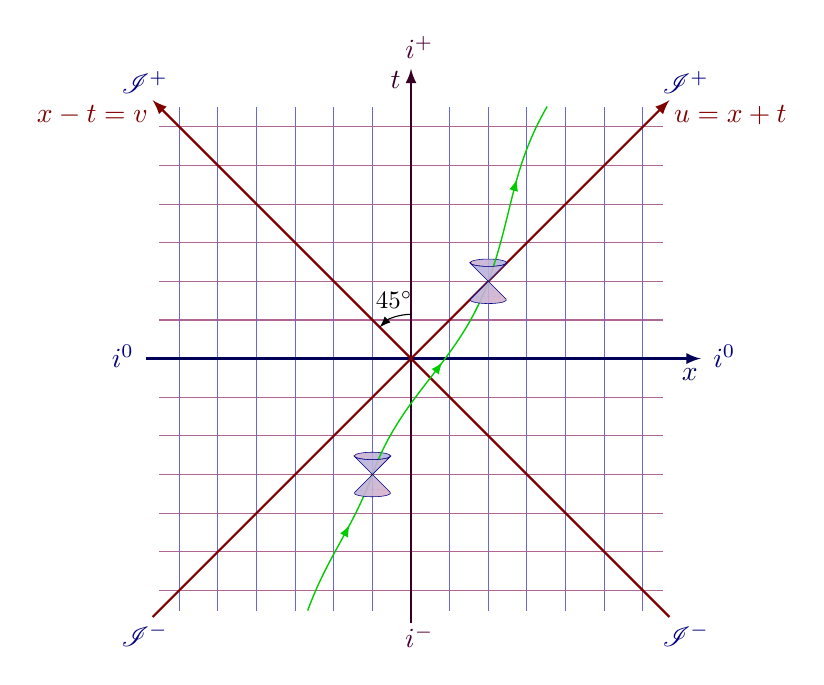
\begin{tikzpicture}[scale=3.2]
  \message{Penrose diagram (45 rotation)^^J}
  
  \def\R{0.10} % size lightcone
  \def\Nlines{6} % number of world lines (at constant r/t)
  \pgfmathsetmacro\d{0.92/\Nlines} % grid size
  
  \coordinate (O) at (0,0);
  \coordinate (W) at (-1.05,0);
  \coordinate (E) at (1.15,0);
  \coordinate (S) at (0,-1.05);
  \coordinate (N) at (0,1.15);
  \coordinate (SW) at (-135:1.45);
  \coordinate (SE) at (-45:1.45);
  \coordinate (NW) at (135:1.45);
  \coordinate (NE) at (45:1.45);
  \coordinate (X0) at (-0.41,-1);
  \coordinate (X1) at (-\d,-3*\d);
  \coordinate (X2) at (2*\d,2*\d);
  \coordinate (X3) at (0.54,1);
  
  % WORLD LINES GRID
  \message{Making world lines...^^J}
  \foreach \i [evaluate={\x=\i*\d;}] in {1,...,\Nlines}{
    \message{  Running i/N=\i/\Nlines, x=\x...^^J}
    \draw[world line]   (-\x,-1) -- (-\x,1);
    \draw[world line]   ( \x,-1) -- ( \x,1);
    \draw[world line t] (-1,-\x) -- (1,-\x);
    \draw[world line t] (-1, \x) -- (1, \x);
  }
  
  % AXES
  \draw[->,thick,mydarkblue!70!black]
    (W) -- (E) node[left=4,below=0] {$x$};
  \draw[->,thick,mydarkpurple!70!black]
    (S) -- (N) coordinate (N) node[below=4,left=0] {$t$};
  \draw[->,thick,mydarkred] (SW) -- (NE) node[below right=-2] {$u=x+t$};
  \draw[->,thick,mydarkred] (SE) -- (NW) node[below left=-2] {$x-t=v$};
  
  \draw pic[->,"$45^\circ$"{above,scale=0.9},draw=black,angle radius=16,
            angle eccentricity=1.0] {angle = N--O--NW};
  
  % INFINITY LABELS
  \node[above=1,left=1,mydarkblue] at (W) {$i^0$};
  \node[above=1,right=1,mydarkblue] at (E) {$i^0$};
  \node[right=3,below=2,mydarkpurple] at (0,-1) {$i^-$};
  \node[right=3,above=0,mydarkpurple] at (N) {$i^+$};
  \node[mydarkblue,left=5,below right=-1] at (SE) {$\calI^-$};
  \node[mydarkblue,right=8,below left=-1] at (SW) {$\calI^-$};
  \node[mydarkblue,left=5,above right=-1] at (NE) {$\calI^+$};
  \node[mydarkblue,right=8,above left=-1] at (NW) {$\calI^+$};
  
  % LIGHT CONE BACK
  \coneback{X1};
  \coneback{X2};
  
  % PARTICLE
  \draw[particle,decoration={markings,mark=at position 0.170 with {\arrow{latex}},
                                      mark=at position 0.505 with {\arrow{latex}},
                                      mark=at position 0.860 with {\arrow{latex}}},postaction={decorate}]
    (X0) to[out=70,in=-110] (X1) to[out=70,in=-110] (X2) to[out=70,in=-120] (X3);
  
  % LIGHT CONE FRONT
  \conefront{X1};
  \conefront{X2};
  
\end{tikzpicture}

\end{document}  